\documentclass{cssspaper}
% \卒論
\修論
% \usepackage{epsbox}
\usepackage{makeidx}
\usepackage{verbatim}
\usepackage[dvipdfmx]{graphicx}
\usepackage{listings,jvlisting}
  \title {調査項目の拡張しやすさを考慮した\\ソースコード解析システムの構築}
   \author{小方 亮人}
   \teacher{香川 考司}
   \chief{香川 考司}
	 \seconda{安藤 一秋}
	 \secondb{高木 智彦}
   \year{令和6年度~(2024年度)}
\date{令和7年1月30日}
% \date{\today}

\lstset{
    basicstyle={\ttfamily},
    identifierstyle={\small},
    commentstyle={\smallitshape},
    keywordstyle={\small\bfseries},
    ndkeywordstyle={\small},
    stringstyle={\small\ttfamily},
    frame=single,
    % framexleftmargin=1em,
    breaklines=true,
    columns=[l]{fullflexible},
   %  numbers=left,
    xrightmargin=3zw,
    xleftmargin=3zw,
    % xleftmargin=3zw,
    numberstyle={\scriptsize},
    % framesep=5pt,
    stepnumber=1,
    numbersep=1zw,
    lineskip=-0.5ex
}

% \makeindex

\begin{etitleenv}
  Implementation of a Source Code Analysis System Considering the Ease
  of Expansion of Survey Items.
\end{etitleenv}

\begin{eabstract}
abstract
\end{eabstract}

\begin{jabstract}
abstract
\end{jabstract}

\begin{keyword}
  Haskell,構文解析,プログラミング学習支援,ソースコード解析
\end{keyword}

\begin{document}
\maketitle
%  \listoffigures % 図の目次
%  \listoftables  % 表の目次

    \chapter{はじめに}
        \section{研究背景}
        大学で情報系の専門課程に進むと、ほとんどの学生がプログラミングの基礎を
        学ぶことになるが、その多くは高校までの学習でプログラミングを経験していることが
        少ないため、初めて本格的なプログラミングを学び始めるということが一般的である。
        初学者がプログラムに関する基礎的なスキルをあっという間に習得することは容易ではなく、
        多くの学生が学習を進める中で自身が記述したコードに関するエラーや警告に対して
        悪戦苦闘することになる。そこで発生したエラーの解決は初学者にとって、
        単なる間違いを直す作業ではなく、問題の本質を理解しその原因を突き止めることが
        重要である。しかしプログラミングを始めたばかりの学習者はエラーの内容が理解できず、
        何が間違っているのかを特定するのに多くの時間を費やしてしまうことが多々ある。
        その結果学習が遅れ、モチベーションの低下を招くことにもつながってしまう。
        中にはコンパイルエラーとして表示されないミスもあり、これらを初学者が自力で
        正確に把握し修正することはとても難しい問題となっている。
        これらのエラーの多くは初学者が陥りやすい些細なミスに起因していることが
        多いため、その修正方法をひとつひとつ丁寧に指導することは学習者にとっても
        教育者にとっても大きな負担となる。このような学習過程において教育者が
        全ての学習者に個別にフィードバックを提供することは難しく、大人数のクラスや
        自己学習環境では特に困難となっている。学習者が自分で改善方法を見つけられない
        状況が続くと、プログラミングに対する苦手意識が強まり、その後の学習にも
        悪影響を及ぼすことになる。したがってプログラミング教育においては、
        学習者が効率的に学び、適切なプログラミング技術を身に着けるための教育支援が
        必要である。特に、間違っている箇所を特定し即座にフィードバックを与え、
        改善方法を迅速に提供することのできるものが効果的であると考えられる。
        このようなフィードバックは学習者が自らコードを改善するための指針を提供し、
        自己修正能力を高めるだけではなく、プログラミング学習に対する自信をも
        促進することが期待される。
        しかし現状ではそのようなコード指摘ツールにはいくつかの課題が存在する。
        多くのツールは専門家向けに設計されており、その出力は初学者にとって
        直感的ではなく理解しづらいものが多いため、そのまま学習者が活用することは
        困難である。また、初学者がよく犯すミスに対して柔軟に対応できるツールの開発が
        求められているが、既存のツールではそのような対応が十分ではなく、
        初学者に適切なフィードバックを提供するための機能が不足している。
        このような背景の中で、初学者に特化したプログラミング学習支援ツールの開発は、
        プログラミング学習の理解を深め、効率的な学習を促進させるために重要な課題である。
        またプログラミング教育における初学者の学習過程では、特に「コードの流れ」に
        対する理解が未熟であることが課題の一つとなっている。
        プログラムは単に記述された命令が順番に実行されるわけではなく、
        制御構文によってその流れが動的に変化するものであるが、
        初学者の中にはこの制御構文を正しく理解できず、何故そのような
        流れになるのかが判断できていなかったり、意図的に利用することが
        難しいと感じてしまったりしている人が多いと感じられる。
        制御構文の理解不足は、コードがどのように動作しているのかが
        理解できなくなる原因となり、その結果としてプログラムの結果が
        予期しないものとなることで効率的なデバッグも行えず、
        学習の進行が遅れることに繋がる。

        そこで、学習者のコードへの指摘を行う支援ツールの開発に取り組んだ研究として、
        C-Helper \cite{1,2,3}や、それを用いた島川の研究 \cite{4}が挙げられる。
        しかしC-HelperではJavaを実装言語として採用し、構文解析の結果として
        得られる抽象構文木を操作するために、Visitorパターンというデザインパターンを
        利用している。この方法では抽象構文木に新しいデータ構造や機能を追加する際に、
        新しいメソッドの追加や各クラスにそのメソッドに応じた実装を追加する必要がある。
        この制約により、C-Helperのアプローチは調査項目の拡張性において課題があると言える。
        また、制御構造の流れを可視化する研究としてLucyらの研究 \cite{5}が挙げられる。
        Lucyらの研究は制御フローグラフによる視覚的フィードバックを用いて
        コードの改善を支援するものであるが、制御フローの可視化のみでは
        どのようにコードを改善するべきか見極めることが困難な場合がある。

        そこで本研究では、学習者に即座にフィードバックを提供することができる
        コード指摘ツールの開発を目標とする。指摘には具体的な改善方針と、
        コードの流れの視覚的なフィードバックが含まれ、学習者のコード改善を支援する。
        指摘するソースコードに用いられる
        プログラミング言語は香川大学の情報系コースのプログラミング講義で
        始めに学習するC言語を対象とする。そして特にコードの流れ、制御構文に
        対して初学者の理解が深まるアプローチを意識する。システム導入に対する
        学習者の負担削減や、プログラムの組込みと修正が容易となるように、
        Webベースでのシステム実装を目指す。

        \section{関連研究}
            \subsection{C-Helper}
            C-Helperは、東京工業大学の内田公太氏によって開発された
            C言語初学者向けの静的解析ツールである。このツールは、
            ソースコード内の問題点を検出し、それを明確で理解しやすい
            エラーメッセージとして提示するだけでなく、解決策も示すことで
            プログラミング学習を支援する仕組みとなっている。
            C-Helperが検出可能なエラー項目は以下のとおりである。
            \begin{itemize}
                \item インデントの不統一
                \item printfのパラメタミス
                \item scanfの値渡しのミス
                \item returnの記述漏れ
                \item char型変数への文字列の代入
                \item 識別子の重複
                \item 定義されていない関数の使用
                \item 構造体におけるセミコロンの記述漏れ
                \item 関数定義の余分なセミコロン
                \item 警告を抑え込むキャスト
                \item メモリリーク
                \item 動的に確保した配列に対するsizeof
                \item ヘッダファイルでの実態定義
            \end{itemize}
            しかし、C-HelperはEclipseのプラグインとして開発されており、
            その導入にはいくつかの課題がある。特に、Eclipse以外の開発環境では
            利用できないこと、さらに特定のバージョンのEclipseでしか
            動作しないことから、広く普及するには技術的および運用上の制約が存在する。

            \subsection{C-Helperを利用したWebベースのC言語開発環境の構築}
            島川の研究では、C-Helper導入における問題点を解消するために、
            C-Helperの機能をWebベースで利用可能な形に改良することが試みられた。
            この研究では、C-HelperがEclipse環境に依存している部分、
            特にライブラリやそのライブラリを使用したメソッドを修正することで、
            ソースコード解析や解析結果の出力をWeb上で実現している。
            この改良により、C-Helperをインストールする際の手間や、
            Eclipseのバージョンに依存する問題を一定程度解消している。
            一方で、このシステムはC-Helperの機能をそのままWeb上に移植する形式で
            実装されているため、C-Helperが対応していないエラー項目については
            新たに実装することができない。また、調査項目を追加する場合、
            C-Helperの本体に変更を加える必要があり、それに伴って本システム側にも
            対応する実装を行う必要がある。これにより、調査項目の拡張には
            多大な手間がかかるという課題が残っている。

            \subsection{CompareCFG: Providing Visual Feedback on Code Quality Using Control Flow Graphs}
            コードの複雑さに関するフィードバック方法を模索し、
            制御フローグラフを用いたツールを開発した研究である。
            制御フローグラフを利用した視覚的フィードバックを与えることで
            学生が改善に向けた行動を取るように促進することを目的としている。
            制御フローグラフとは以下の図\ref{fig:flow}のようなものであり、コードの制御構造を視覚的に表現し、
            各命令や分岐がどのように接続されているかを示している。
            \begin{figure}[h]
                \centering
                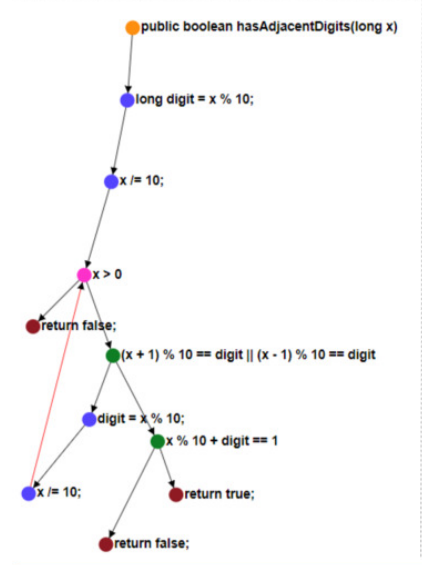
\includegraphics[width=7cm]{flow.png}
                \caption{制御フローグラフ}
                \label{fig:flow}
            \end{figure}

            制御フローグラフは、構造を視覚的に表現できる手法として
            プログラム分析やコンパイラ設計の分野で利用されている。
            コードの流れを直感的に把握できるため、デバッグや最適化、プログラム検証などで
            活用されている。教育の分野でも、学生がコードの流れを理解しやすくするための
            ツールとして注目されている。制御フローグラフによるフィードバックを与えることで、
            学生がよりシンプルで効率的なコードに改善でき、その後の課題で
            コーディングスキルや自己修正能力が向上したことが示されている。
            このことから、視覚的フィードバックを提供することで学生がコードの改善点をより
            理解しやすくなることが考えられる。しかし視覚的フィードバックだけでは学習者が
            それを見てどのようにコードを改善していくかの方針を考えることが困難な場合が
            あるため、具体的な改善方針が含まれるフィードバックを組み合わせる必要がある。

        \section{Webベースシステムの利点}
        本研究で開発したシステムは、Webページを通じてソースコードを送信し、
        解析結果をその場で表示するWebベースのアプローチを採用している。
        Webベースシステムにすることにより、利用者に対して以下のような
        利便性を提供できる。

        \begin{itemize}
           \item システムのインストールや初期設定が不要
           \item インターネット環境があれば、どのデバイスからでもアクセス可能
           \item 常に最新のシステム機能を利用できるため、手動でのアップデートが不要
        \end{itemize}

        また、開発者側にも以下のような利点が考えられる。

        \begin{itemize}
           \item システムのインストール方法やセットアップ手順の説明が不要
           \item ソフトウェアの改善や不具合修正が迅速に反映できるため、ユーザーへの対応が容易
        \end{itemize}

        これにより、システム導入に関する障壁が大幅に減少し、どんな学習者でも手軽に
        利用できる環境を整えることができる。特に技術的な設定が不要なため、利用者は
        煩わしさを感じることなくシステムを活用することができる点が大きな利点である。

        \section{静的解析の利点}
        本研究のシステムでは、ソースコードに対して静的解析を実施する。静的解析とは、
        ソフトウェアを実行せずにソースコードを解析する手法であり、実行時に
        問題を発見する動的解析とは異なる。静的解析を利用することにより、
        コードの記述段階でエラーを早期に発見でき、実行前に改善を加えることが
        可能となる。さらに、静的解析は学習者がインデント等のコードの品質を高めることに
        繋げるための支援にもなり、コードの整合性や可読性の向上にも貢献する。
        これによってコードの誤読や理解の誤りを防ぐことができ、
        予期しないバグやエラーの修正も効率的に行えるメリットがある。

        \section{本研究に求められること}
        これらの点を踏まえて、本システムに求められる要件は以下のとおりである。
        \begin{itemize}
            \item 初学者向けの静的解析を行うことができる
            \item 学習者に即座にフィードバックを行うことができる
            \item コードの流れの理解を支援することができる
            \item 調査項目の拡張性が期待できる
            \item Webベースのシステムである
        \end{itemize}
        プログラミング初学者が、自身のソースコードのどの部分に問題があり、
        何が原因でエラーになっているのか、また修正方法について理解し
        判断できるようにするため、初学者が直面しやすいエラーに対応した
        ソースコード解析を行い、即座にフィードバックを提供するシステムが
        求められる。このシステムは、学習効率を向上させるだけでなく、
        学習者がコードの流れや構造を正しく理解できるよう支援することを目指す。
        さらに、運用の中で新しいエラーや課題が発生した際、
        それらを柔軟に追加・拡張できるようにシステムを実装することで、
        システムの対応範囲を広げ、学習者の多様なニーズに応えることが
        可能となる。これにより、利用者が増加し、より多くの学習者に
        貢献することが期待される。学習者が気軽に利用できるように、
        システムをWebベースで実装することで、アクセス性を向上させることが必要である。

        \section{章構成}
        本論文の構成は以下のようになっている。
        第2章で本システムを実装するにあたって使用した技術について説明する。
        第3章では実装したシステムについて述べる。
        第4章では本システムの試用実験と評価について述べる。
        第5章で本論文のまとめと課題点について述べる。

    \chapter{使用技術}
    ここでは本システムで使用した技術について説明する。

        \section{Haskell}

            \subsection{Haskellとは}
            Haskellは、関数型プログラミング言語の一つであり、
            計算や処理を関数の組み合わせとして数学的に表現し、
            記述することを特徴としている。この言語は、記号論理学者である
            Haskell Brooks Curry氏の名前にちなんで名付けられている。
            現在、Haskellの主な処理系としては、
            GHC (Glasgow Haskell Compiler) が広く使用されている。
      
            \subsection{Haskellの特徴}
            Haskellは関数型言語に特有の機能を数多く備えており、
            参照透過性や遅延評価に加え、パターンマッチや型推論
            などの特徴を持っている。
            これらの機能を組み合わせることで、命令型言語に比べて
            Haskellはより簡潔かつ効率的にコードを記述できる場合が多く、
            特に構文解析やデータ処理の分野でその強みを発揮する。
            以下にHaskellの代表的な特徴をいくつか示す。
            \begin{itemize}
                \item 参照透過性
            
                C言語やJavaなどの命令型言語では、課題解決のために
                命令や手続きを組み合わせて記述する。このアプローチでは、
                システムの状態が命令の実行によって変化するため、
                複数の処理が同じ変数を参照している場合、
                予期しない結果が生じることがある。このような現象は
                「副作用」と呼ばれ、デバッグやメンテナンスの複雑化を招く
                要因となる。一方、Haskellを含む関数型言語では、
                プログラムの目的に沿った関数を定義することで記述を進め、
                副作用を極力排除する設計思想が採用されている。
                特にHaskellは「参照透過性」という性質を持ち、
                同じ引数で呼び出した関数が常に同じ結果を返す。
                この数学的な特徴により、プログラムの挙動が予測可能となり、
                安全性と信頼性が向上する。また、参照透過性は関数のテストや
                再利用を容易にし、大規模なコードベースにおいても
                品質を維持する重要な要素となる。

                \item 遅延評価
            
                一般的なプログラミング言語では、関数を呼び出す際、
                引数が事前に評価され、その結果が関数に渡される
                「正格評価」が採用されている。一方、Haskellでは
                「遅延評価」という特性があり、引数の値が実際に必要に
                なるまで評価が行われない。この特性は関数の引数だけでなく、
                変数の値を参照する際にも適用される。遅延評価の利点として、
                無限リストのような無限データ構造を扱える点が挙げられる。
                例えば、以下のコードでは無限リストを生成し、
                必要な部分だけを取り出して計算を行うことができる。

                \begin{lstlisting}
                take 5 [1..]
                -- 結果: [1, 2, 3, 4, 5]
                \end{lstlisting}

                この仕組みにより、必要最小限の計算だけが実行されるため、
                計算効率が向上し、プログラムの柔軟性を高めることができる。
                例えば条件分岐で実際に使用されない計算を
                スキップすることができる。ただし、遅延評価には注意点も
                ある。計算が後回しにされるため、大規模なデータ構造を
                扱う場合にメモリ使用量が予想外に増加するリスクがある。
                そのため、遅延評価の特性を理解し、適切に設計することが重要である。

                \item パターンマッチ
                
                Haskellでは、関数定義においてパターンマッチを
                利用することで、入力引数に応じた条件分岐を簡潔に記述できる。
                この機能はコードの可読性を向上させるとともに、
                安全で明確なプログラムの構築を可能にする。
                関数呼び出し時には関数定義内のパターンが上から順に評価され、
                最初にマッチしたパターンに対応する処理が実行される。
                マッチするパターンが存在しない場合にはエラーが発生する。
                以下に階乗を計算する関数の例を示す。

                \begin{lstlisting}
                fact 0 = 1
                fact n = n * fact (n - 1)
                \end{lstlisting}

                この関数は、引数が0の場合に1を返す。引数が0以外の
                任意の値の場合はnに値が束縛され、再帰的に
                fact (n - 1) を呼び出して計算が進行する。
                パターンマッチを用いることで、複雑な条件分岐を簡潔に
                記述することができる。この特徴によりコード全体の
                可読性が向上し、結果として保守性も高まる。
                特に条件分岐が多い場合でも分かりやすい記述が可能であり、
                プログラムの設計や実装が容易になる。さらに、
                パターンマッチはプログラムの安全性を向上させる役割も果たす。
                未対応のケースが存在する場合、コンパイル時に警告が表示されるため、
                プログラマは問題を事前に発見しやすくなる。
                ワイルドカードなどを活用することで、
                すべてのケースを網羅的に記述することが可能となり、
                プログラムの信頼性が高まる。このように、
                パターンマッチは効率的で安全なプログラミングを支える重要な機能である。

                \item 型推論
            
                Haskellの型推論機能は、プログラマに対して
                静的型付けの利点を提供しつつ、
                コードの簡潔さと可読性を高めるものである。
                静的型付けはコンパイル時にエラーを事前に発見できるという
                メリットを持つ一方で、データ型を明示的に指定する必要があり、
                プログラムの複雑さや冗長さを招く可能性がある。
                一方、動的型付けではデータ型を指定する手間が省けるが、
                エラーが実行時まで発見されないというデメリットを伴う。
                Haskellの型推論は、これらの両者の短所を補完するよう
                設計されている。型推論により、プログラマはデータ型を
                明示的に指定する必要がなく、与えられたコードから
                コンパイラが自動的に型を推測し、適切に判断する。
                これによりプログラムの記述は簡潔になり、
                複雑な型指定による冗長さを回避できる。
                さらに型推論の機能は、コンパイル時にコードの正確性を
                保証する点で非常に有効である。
                明示的な型指定が不要でありながら、
                静的型付けと同様にコンパイル時にエラーを検出できるため、
                コードの安全性を確保し、エラーの発生を抑えることが可能となる。
                これによりHaskellのプログラミング環境は、
                簡潔なコード記述とエラー抑制の両立を実現している。

                \item モナド
                
                モナドは、Haskellにおいてプログラムの副作用を安全かつ
                体系的に扱うための枠組みである。ここでいう副作用とは、
                状態の変更を伴う破壊的代入や入出力操作など、
                プログラミングにおける一般的な副作用を指す。
                モナドは、これら副作用を伴う処理を共通の構造を通じて
                抽象化し、その構造に基づいた演算子を用いることで一貫して
                扱うことを可能にする。これにより、副作用を安全に
                管理するための強力なツールを提供している。
                特にHaskellで頻繁に使用されるモナドの一つがIOモナドであり、
                主に入出力操作に関連する役割を担う。IOモナドを用いることで、
                標準入力や標準出力といった外部とのやり取りを安全に
                記述することが可能である。以下に、IOモナドを用いた
                プログラムの例を示す。

                \begin{lstlisting}
                main :: IO ()
                main = do
                            line <- getLine
                            putStrLn line
                \end{lstlisting}

                このコードでは、getLineによって標準入力から文字列を取得し、
                それを変数lineに束縛している。その後、putStrLn関数を用いて、
                取得した文字列を標準出力に表示する。putStrLnは文字列String型
                を引数として受け取り、標準出力への表示を行うIOアクションを返す
                関数である。このように、IOモナドを用いることで、
                外部とのやり取りを明確に区別しながら副作用を管理することができる。

            \end{itemize}
            Haskellにはこれらのような特徴があり、構文解析やデータ処理では、
            抽象構文木の操作や再帰的な処理が頻繁に求められるが、これらは
            Haskellの強みであるパターンマッチや型システムなどを
            活用することで効率的かつ安全に実現できる。

        \section{language-c-quote}
        language-c-quoteはHaskellのライブラリであり、
        一般的なC言語のパーサを提供している。
        language-c-quoteは構文解析の結果が扱いやすいため、
        新しく調査項目を増やす際に容易にプログラムを
        追加することができると考え本システムの構文解析に用いている。
        Haskellとの親和性が高く、構文解析結果をそのままHaskellの型で扱える点や、
        実装コストが低く、C言語の複雑な構文規則にも対応済みである点も利点である。
        以下に実際にC言語のソースコードを解析した結果を載せる。
        その解析結果から調査したい構文等を抜き出し真偽を確かめている。
        \begin{figure}[h]
            \centering
            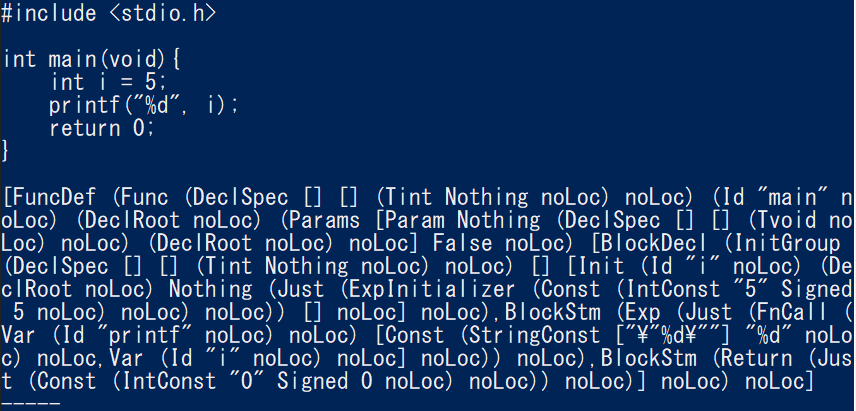
\includegraphics[width=15cm]{lcq.png}
            \caption{language-c-quoteによるソースコードの解析結果}
            \label{fig:lcq}
        \end{figure}

        \section{Mermaid.js}
        Mermaid.jsは、テキストベースでフローチャートやシーケンス図、
        ガントチャートなどのダイアグラムを記述・生成できるJavaScriptライブラリである。
        Markdown形式のようなシンプルな構文でダイアグラムを定義できるため、
        プログラムやドキュメント内での利用が容易であり、視覚的な情報表現を手軽に実現する。
        本システムでは、Mermaid.jsを利用してC言語の制御構文を視覚化し、
        初学者がコードの流れを直感的に理解できるように設計した。
        Mermaid.jsを採用した主な理由は以下の通りである。
        \begin{itemize}
            \item コードを直接グラフ構造に変換するためのシンプルな文法を持つ。
            \item ブラウザ上での即時描画に対応し、Webベースシステムとの親和性が高い。
            \item 制御フローやロジックをフローチャート形式で分かりやすく表示可能。
        \end{itemize}
        以下はMermaid.jsによるフローチャート生成の例である。
        \begin{lstlisting}
            graph LR
            A --> B
            B -- 条件が真 --> C
            B -- 条件が偽 --> D
            C --> E
            D --> E
        \end{lstlisting}
        \begin{figure}[h]
            \centering
            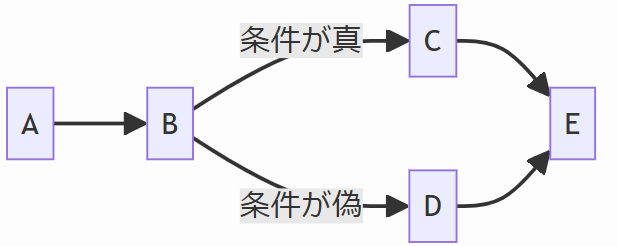
\includegraphics[width=13cm]{mermaid.png}
            \caption{Mermaid.jsによるフローチャート生成}
            \label{fig:mermaid}
        \end{figure}

        このような視覚化により、初学者がコードの論理構造を容易に理解できる環境を提供している。

        \section{CodeMirror}
        CodeMirrorは、ブラウザ上で動作するコードエディタで、
        複数のプログラミング言語に対応しており、シンタックスハイライト、
        オートコンプリート、エラー表示などの機能を提供する。
        本システムではCodeMirrorを活用して、学習者が入力したコードに
        対してエラー箇所をハイライトすることで直感的に
        把握できるようにするために利用している。
        エラー箇所ハイライト機能はコードの文法エラーや
        警告が発生した位置を視覚的に示すことができる。
        エラーが発生した行に色付けを行うことで、
        誤った部分を強調し効率的に学習支援を行う。
        これにより、学習者は自分のコードの問題をすぐに認識し、
        修正を行うことができる。

    \chapter{システムの実装}
    ここでは本システムについて実際の実行画面を踏まえて詳細に述べる。
        \section{システムの概要}
        本システムは、主にプログラミング講義で学習者が提出する、
        課題に対して記述されたコードを対象とし、
        そのコードを解析して学習者にフィードバックを提供することを目的として構築する。
        ソースコードを構文解析してデータを読み取り、ある構造の特定や指摘に利用する。
        対象とする言語は、香川大学で初めに学習するC言語のソースコードとする。
        システムの全体図としてはこのようになっている。

        \begin{figure}[h]
            \centering
            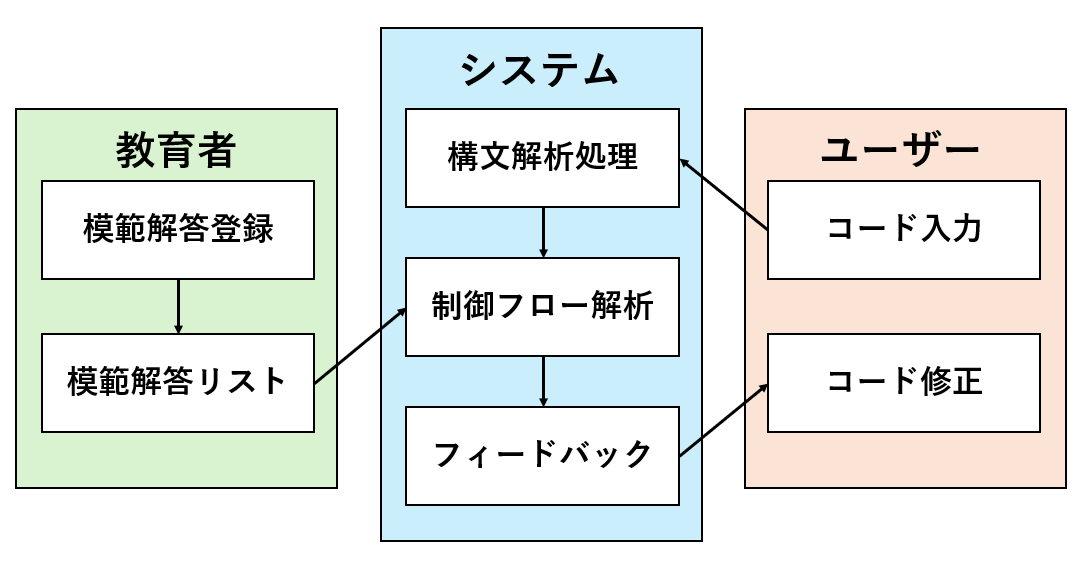
\includegraphics[width=13cm]{system.png}
            \caption{システム全体図}
            \label{fig:system}
        \end{figure}

        まず学習者がブラウザ上でソースコードを入力し、
        それをシステムが受け取って構文解析を行う。
        解析によりコードの構造を自動的に検出し、解析結果とフィードバックを即時に
        ブラウザ上に出力する。フィードバックがすぐに与えられることで学習者は
        その場でコードの修正に取り組むことができる。また、Webアプリケーションとして
        実装することでインストールなどの手間を省き、学習者にとって利用しやすく、
        自己学習の効率を向上させることができるシステムを構築する。
        学習者へのフィードバックとしては、制御フローの視覚的フィードバックと、
        テキストメッセージを組み合わせることによって問題点や改善点を示すことで、
        より具体的な改善方針を学習者に与え、初学者でも理解しやすいフィードバックを目指す。
        視覚的フィードバックにより、分岐やループなどの複雑な部分を
        直感的に把握できるようにし、メッセージによって具体的な問題個所や改善のための
        アドバイスなどを詳細に説明することができる。
        また本システムではプログラミング教育における利用を考慮し、
        学習者が課題に対して提出するために記述したコードと
        模範解答の解析結果を比較する機能を提供する。
        教育者が模範解答のファイル名とコードを登録することで、
        学習者側からは登録されている模範解答リストを確認することができる。
        模範解答のファイル名に応じた個別の解析ページにアクセスすることができ、
        自身のコードと模範解答のコードの制御フローを比較することができる。
        この制御フローの比較により、自身のコードの複雑な構造や冗長な部分を
        直感的に把握することができ、より簡潔で効率的なプログラムを
        記述するための支援が行われる。

        \section{ソースコードの解析}
        解析にはプログラミング言語Haskellを利用する。
        Haskellは、純粋関数型プログラミングの特徴を持ち、
        関数の再利用や組み合わせによってシステム全体を柔軟に構築することに優れている点や、
        高い抽象化能力により、複雑な解析結果もシンプルに扱うことができる点がある。
        それらを利用することにより、特に、既存の関数やモジュールを組み合わせることで、
        新しい機能を柔軟に拡張できる点が強みとなる。
        またHaskellは強力な静的型システムによりコンパイル時に型の安全を確認できるため、
        機能の拡張に伴うリスクを最小限に抑え、堅牢で信頼性の高い解析機能を
        実現することができる。
        本システムは、Haskellを使用してC言語のソースコードを読み取り、
        language-c-quoteを活用して構文解析を行う。
        解析されたコードはMermaid形式に変換され、
        制御構文の流れを視覚化したグラフとしてブラウザ上に即座に描画される。
        この機能により、初学者がコードの動作や流れをフローチャートのような形式で
        直感的に把握することを支援する。
        Haskellのライブラリであるlanguage-c-quoteを用いた構文解析について、詳しく述べる。

        \begin{lstlisting}
        import Language.C
        import Data.ByteString.UTF8 as UTF8 (fromString)

        parseProg :: String -> Either SomeException [Definition]
        parseProg str = parse [C11] [] parseUnit (UTF8.fromString str) Nothing
        \end{lstlisting}

        上記のparseProgのような関数を作成し、引数strとしてソースコードの
        文字列を渡すことで構文解析が行われる。
        実際に以下のソースコードを解析した結果を載せる。

        \begin{lstlisting}
        #include <stdio.h>
            
        int main(void){
            int i = 5;
            if (i == 5) {
                printf("%d", i);
            }
            return 0;
        }
        \end{lstlisting}

        \begin{figure}[h]
            \centering
            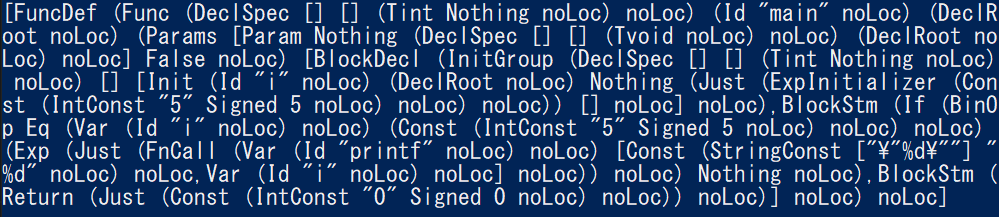
\includegraphics[width=13cm]{lcq1.png}
            \caption{language-c-quoteで解析した結果}
            \label{fig:lcq1}
        \end{figure}

        このような解析結果から調査したい構文や変数等を
        抜き出すことで真偽の判定を行っている。
        解析されたソースコードの結果から特定の構文や変数情報を抽出し、
        その正確性を検証している。以下に、図示した解析結果を用い、
        if文やprintfの情報を抽出する手順を説明する。

        language-c-quoteで解析された結果を適切に読み取るためには、
        解析結果に含まれる複数のデータ型とその構成を理解することが
        重要である。データ型の詳細はLanguage.C.Syntaxに
        記載されており、例えば図の初めのFuncDefの構成は
        FuncDef Func !SrcLocとなっている。このように解析結果を参照しながら
        目的の構文を特定していく。
        if文の情報は、解析結果の5行目に該当するBlockStmから始まる部分に見つかる。
        このデータ型はStmを基礎としており、StmがIfの形を取る場合、
        その構成はIf Exp Stm (Maybe Stm) !SrcLocとなる。
        このExpには次のような解析結果が含まれている。

        \begin{lstlisting}
            BinOp Eq (Var (Id "i" noLoc) noLoc) (Const (IntConst "5" Signed 5 noLoc) noLoc) noLoc
        \end{lstlisting}

        このBinOp Eqは、変数iと定数5の等価性を示しており、
        元のソースコードにおけるif文の条件式(i == 5)に対応している。
        同様に、if文内部のprintfについては、以下のように解析がされている。
        \begin{lstlisting}
            Exp (Just (FnCall (Var (Id "printf" noLoc) noLoc) [Const (StringConst ["\%d"] "\%d" noLoc) noLoc, Var (Id "i" noLoc) noLoc] noLoc)) noLoc
        \end{lstlisting}
        これに基づき、printfの情報を抽出し、条件式やパラメータのミスを検出する。
        本システムでは、上記の方法に基づいて他の構文についても
        同様の処理が可能である。Language.C.Syntaxの構造を理解し、
        Haskellのコードを記述することで、新たな調査項目への対応が容易となる。
        この点において、システムの拡張性が保証されているといえる。


        \section{筆者の先行研究}
        本システムのエラー検出機能は、筆者が過去に開発したWebアプリケーションシステムを
        利用している。この過去のシステムでは、プログラミング初学者が陥りやすい構文的なミスや
        論理的な誤りを検出し、学習支援を行うことを目的としており、その詳細については
        先行研究 \cite{6}で述べている。
        そのシステムで検出できるエラー項目は以下のとおりである。
        \begin{itemize}
            \item インデントのミス
            \item printfの変数の数が間違っているミス
            \item scanfの変数の数が間違っているミス
            \item if文の条件式が関係演算子ではなく代入式になっているミス
            \item 関数名が他の関数と重複しているミス
            \item 返却値がint型の関数にreturnが記述されていないミス
        \end{itemize}
        本研究では、このエラー検出システムを基盤として利用しつつ、
        C言語の制御構文をフローチャートの形で可視化し、コードの流れを
        より理解しやすくなるように改良を加えている。

        \section{解析可能な項目}
        本システムでは制御構文をグラフ上に可視化している。
        対応している制御構文と描画されるグラフの例を示す。

            \subsection{If文}
            \begin{lstlisting}
                #include <stdio.h>

                int main() {
                    int num = 10;
                    if (num > 0) {
                        printf("正の数です。");
                    }
                    return 0;
                }
            \end{lstlisting}

            グラフ上での表示は以下の図\ref{fig:if}のとおりである。

            \begin{figure}[h]
                \centering
                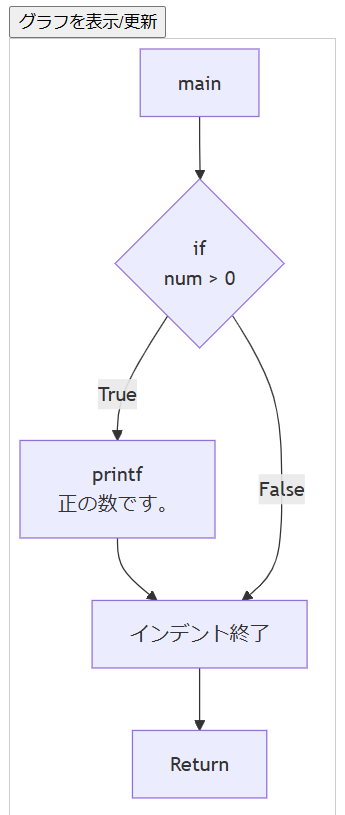
\includegraphics[width=6cm]{if.png}
                \caption{if文の描画例}
                \label{fig:if}
            \end{figure}

            \subsection{For文}
            \begin{lstlisting}
                #include <stdio.h>

                int main() {
                    for (int i = 0; i < 5; i++) {
                        printf("%d", i);
                    }
                    return 0;
                }
            \end{lstlisting}
            グラフ上での表示は以下の図\ref{fig:for}のとおりである。

            \begin{figure}[h]
                \centering
                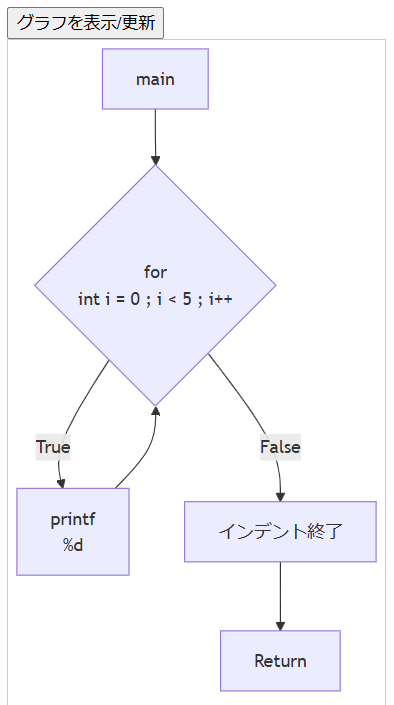
\includegraphics[width=8cm]{for.png}
                \caption{for文の描画例}
                \label{fig:for}
            \end{figure}

            \subsection{While文}
            \begin{lstlisting}
                #include <stdio.h>

                int main() {
                    int i = 0;
                    while (i < 5) {
                        printf("%d", i);
                        i++;
                    }
                    return 0;
                }
            \end{lstlisting}

            グラフ上での表示は以下の図\ref{fig:while}のとおりである。
            
            \begin{figure}[h]
                \centering
                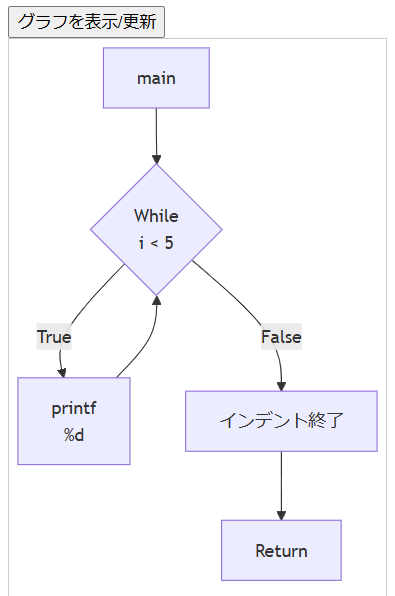
\includegraphics[width=8cm]{while.png}
                \caption{while文の描画例}
                \label{fig:while}
            \end{figure}。

            \subsection{Do-While文}
            \begin{lstlisting}
                #include <stdio.h>

                int main() {
                    int i = 0;
                    do {
                        printf("%d", i);
                        i++;
                    } while (i < 5);
                    return 0;
                }
            \end{lstlisting}

            グラフ上での表示は以下の図\ref{fig:dowhile}のとおりである。

            \begin{figure}[h]
                \centering
                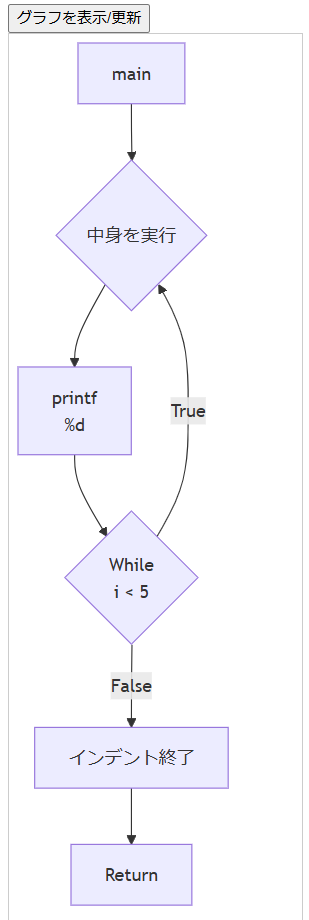
\includegraphics[width=4cm]{dowhile.png}
                \caption{do-while文の描画例}
                \label{fig:dowhile}
            \end{figure}

        \section{システムの実行}
        本システムはWebページにアクセスすることでシステムを利用できる。
        システムページにアクセスすると、入力フォームが表示される(図\ref{fig:systemuse1})。
        
        \begin{figure}[h]
            \centering
            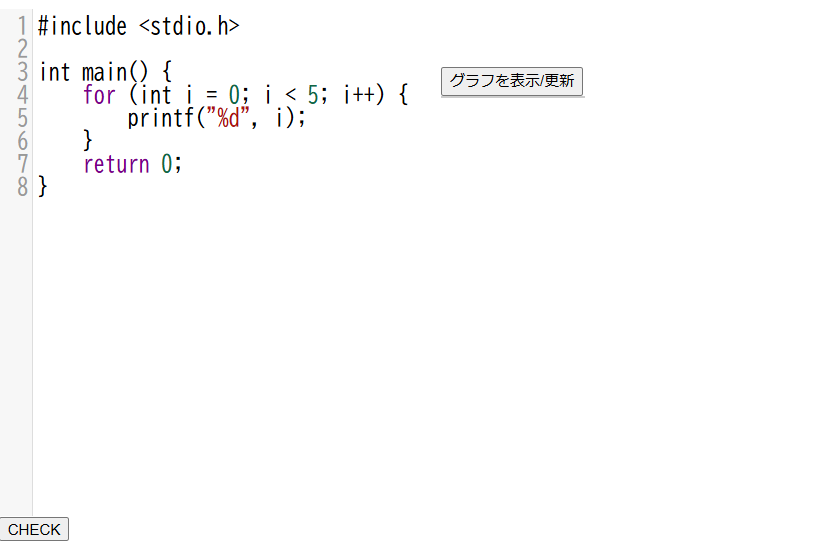
\includegraphics[width=10cm]{systemuse1.png}
            \caption{ソースコード入力画面}
            \label{fig:systemuse1}
        \end{figure}

        表示されているテキストエリアに解析したい
        ソースコードを入力し、CHECKボタンを押すことで
        Haskellプログラムに文字列として
        ソースコードが送信され、構文解析が行われる。
        そして解析した結果とエラーの箇所や内容、
        生成した制御フローグラフの表示が行われる。
        結果表示の際にはエラーがある行番号の色を変更することで強調している。
        実際にソースコードを入力した際の結果表示画面を以下に示す(図\ref{fig:systemuse2})。

        \begin{figure}[h]
            \centering
            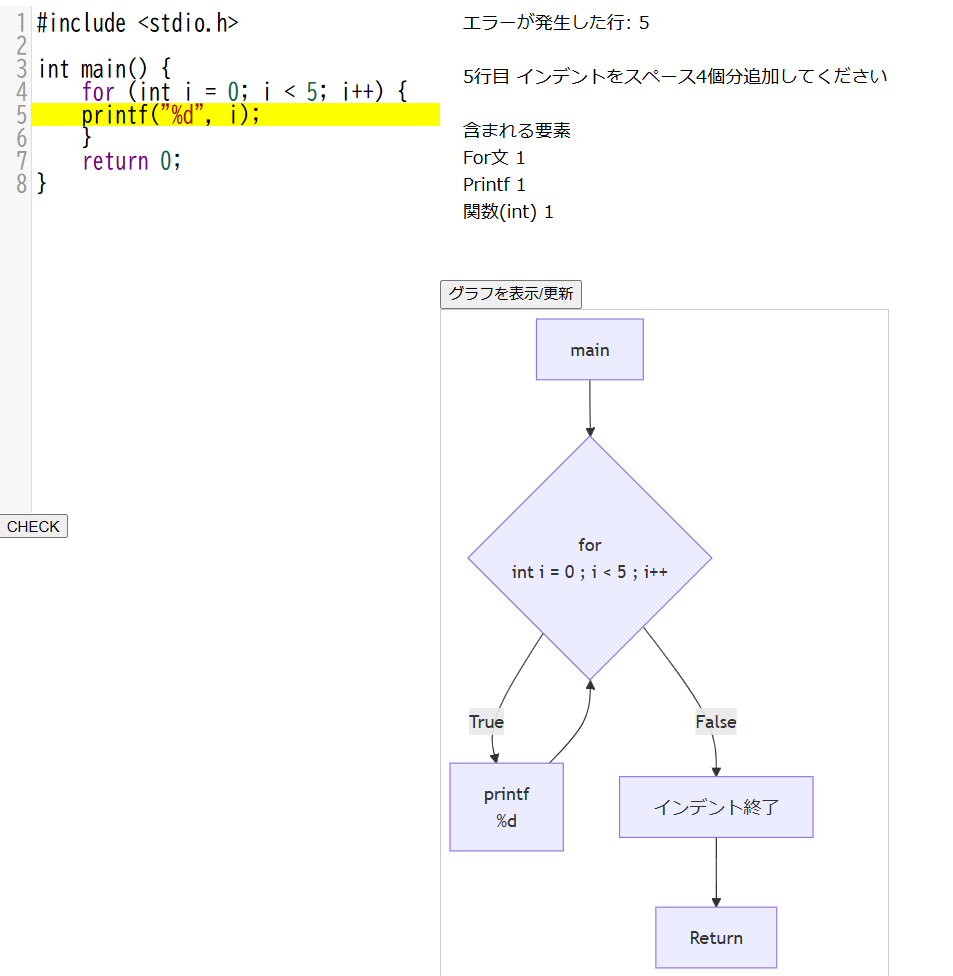
\includegraphics[width=10cm]{systemuse2.png}
            \caption{解析結果表示画面}
            \label{fig:systemuse2}
        \end{figure}

        解析結果の表示画面では特に初学者がソースコードのエラーを
        修正できるように分かりやすくエラー内容を表示することを意識している。
        エラーがある行はCodeMirrorを利用しハイライトすることで
        一目で間違っている行を理解することができる。
        通常のコンパイラでは文字情報でしかエラー内容が示されていないため、
        視覚的にエラー箇所を理解することができない。
        また、画面右側では生じているエラーの内容について行番号と共に記している。
        エラーによっては修正するために何を行えば良いかの表示もしており、
        表示を見てすぐにエラーの修正を行うことができる。
        解析を行うことでコードのグラフを表示することが可能となり、
        描画されたグラフを確認することでコードの制御構造による流れを
        可視化し、学習者の理解を促進させる支援を行う。




    \chapter{システムの試用実験と評価}
    ここでは、システムの試用実験と評価について述べる。

    \chapter{結論}
        \section{まとめ}

        \section{今後の課題}
    

\acknowledgment  % 謝辞

\begin{thebibliography}{99} % 参考文献

\bibitem{1}
サイボウズ・ラボユース Ucida Kota, ``C-Helper GitHub'',
    
https://github.com/uchan-nos/c-helper (閲覧日:2023年2月)
    
\bibitem{2}
内田 公太, 権藤 克彦, ``C言語初学者向けツールC-Helperの現状と展望'',
    
第54回プログラミングシンポジウム予稿集, pp.153-160, 2013
    
\bibitem{3}
内田 公太, 権藤 克彦, ``C言語初学者向けツールC-Helperの予備評価'',
    
電子情報通信学会技術研究報告=IEICE technical report:信学技報, 巻113, 号159, pp.67-72, 2013

\bibitem{4}
島川 大輝, 香川 考司, ``C-Helperを用いたWebベースのC言語開発環境の構築'',

教育システム情報学会第40回全国大会 (JSiSE2015) 講演論文集, A3-1, 2015.

\bibitem{5}
Lucy Jiang, Robert Rewcastle, Paul Denny, Ewan Tempero, 
``CompareCFG: Providing Visual Feedback on Code Quality Using Control Flow Graphs''

ITiCSE '20: Proceedings of the 2020 ACM Conference on Innovation and Technology in Computer Science Education, Pages 493-499, June 2020

\bibitem{6}
小方 亮人, 香川 考司, ``調査項目の拡張しやすさを考慮したソースコード解析システムの構築'',

教育システム情報学会第48回全国大会 (JSiSE2023) 講演論文集, E3-4, 2023.


\end{thebibliography}


\end{document}
